%%%%%%%%%%%%%%%%%%%%%%%%%%%%%%%%%%%%%%%%%%%%%%%%%%%%%%%%%
\part{Introduction aux projets existants}
\chapter[Présentation de l’approche Arduino]{Présentation de l’approche Arduino}
\label{chap:chap2}

\section{Qu'est-ce qu'Arduino?}

\begin{figure}[h]
\begin{center}

\includegraphics[scale=0.4]{../images/Arduino/Arduinologo.png}
\caption{Logo Arduino}
\end{center}
\end{figure}

Le système Arduino \footnote{Le projet Arduino a reçu un titre honorifique à l'Ars Electronica 2006, dans la catégorie Digital Communities}
est une plateforme \textit{open-source} de programmation embarquée basée sur une carte à microcontrôleur de la famille AVR\footnote{
Cœur du processeur et famille de microcontrôleurs}, et sur un environnement
de développement intégré qui permet d'écrire, compiler et transférer un programme vers la carte. Ce logiciel utilise la technique du Processing/Wiring
\footnote{Processing est un langage de programmation et un environnement de développement}.

Avec le système Arduino on peut réaliser divers tâches, par exemple le développement des objets interactifs indépendants: le prototypage rapide. Aussi,
la domotique, qui grâce aux différents interrupteurs/capteurs permet de contrôler plusieurs sorties matérielles: contrôle des appareils domestiques,
pilotage de robot, etc \ldots ou même charger des batteries par l'analyse et la production des signaux éléctriques.
De plus, il peut communiquer avec des logiciels tournant sur l'ordinateur tel que Macromedia Flash, Processing, MaxMSP, etc \ldots.

Le langage de programmation Arduino est une implémentation de Wiring, une plateforme de développement similaire, qui est basée sur l'environnement
multimédia de programmation Processing.

Les cartes électroniques sont accesibles a tous, elles peuvent être achetées pré-assemblées ou être fabriquées manuellement, tout en ayant la totalité des
informations nécessaire à l'assemblage.

\section{Avantages d'utilisation de Arduino}

Le système Arduino a simplifié la façon de travailler avec les microcontrôleurs, en offrant plusieurs avantages pour les enseignants, les étudiants et
les amateurs intéressés par d'autres systèmes. Ce système prend en charge des détails compliqués de la programmation des microcontrôleurs et les intègrent
dans une présentation facile à utiliser. Voici, plusieurs avantages que propose Arduino:

\begin{description}
 \item[Peu coûteux:] En comparaison à d'autres plateformes les cartes Arduino sont peu coûteuses, les moins chères sont les versions qui peuvent être
assemblées à la main.
 \item[Multi-plateforme:] Le logiciel de programmation des modules Arduino est une application Java, libre et qui peut tourner dans plusieurs systèmes
d'exploitation tel que Linux, Windows et Mac.
 \item[Environnement de programmation clair et simple:] Le logiciel est facile à utiliser pour les débutants ( nous avons eu l'occasion de le tester lors de
l'initiation à l'Arduino proposé par Olivier Richard); tout en restant flexible pour des utilisations avancées.
 \item[Logiciel Open Source et extensible:] Le logiciel et le langage Arduino sont publiés sous licence Open Source et sont donc disponible à tous, ce qui
offre la possibilité de compléter et/ou améliorer le projet. Le langage Arduino, qui utilise le langage C++, peut être étendu grâce aux librairies C++.
 \item[Matériel Open Source et extensible:] La version sur plaque d'essai de la carte Arduino peut être achetée à très bas coût et peut être montée par
n'importe quel utilisateur, elle a pour but de comprendre comment la carte fonctionne. De plus, tous les schèmas de modules Arduino sont publiés. Dès lors, les
utilisateurs plus experimentés en embarqué peuvent apporter des améliorations à leurs montages.
\end{description}


\section{Utilisation d'Arduino}

  Dans cette partie on va décrire certains points importants pour l'utilisation du logiciel, de la carte et du langage Ardduino.

\begin{figure}[h]
\begin{center}
 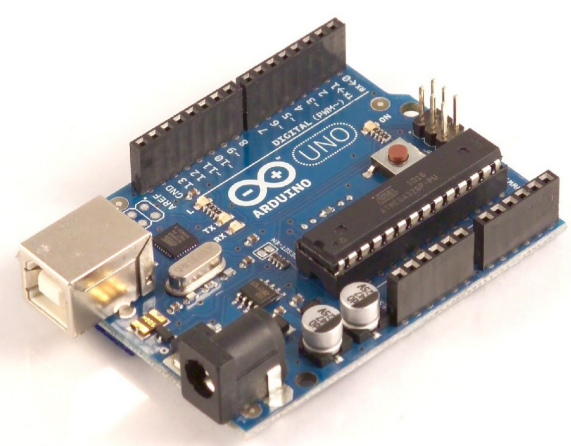
\includegraphics[scale=0.4]{../images/Arduino/arduinoUno.png}
\caption{Carte Arduino Uno}
\end{center}
\end{figure}

Un programme en langage Arduino doit obligatoirement être composé de ces deux fonctions:
\begin{itemize}
 \item la fonction d'initialisation $setup()$ qui est exécutée une seule fois au démarrage.
 \item la fonction "boucle sans fin" loop() qui est exécutée en boucle une fois que la fonction setup() a été exécutée une fois.
\end{itemize}

Puis, si besoin, autres fonctions peuvent être crées en suivant ce schèma:
\begin{table}[h]
\begin{lstlisting}
type nom_fonction (arguments) {
   // ici le code de la fonction
}
\end{lstlisting}
\caption{Création d'une nouvelle fonction en Arduino}
\end{table}


\begin{table}[h]
\begin{lstlisting}
/*
  Blink
  Turns on an LED on for one second, then off for one second, repeatedly.
*/
void setup() {
  // initialize the digital pin as an output.
  // Pin 13 has an LED connected on most Arduino boards:
  pinMode(13, OUTPUT);
}

void loop() {
  digitalWrite(13, HIGH);   // set the LED on
  delay(1000);              // wait for a second
  digitalWrite(13, LOW);    // set the LED off
  delay(1000);              // wait for a second
}
\end{lstlisting}
\caption{Exemple Blink pour Arduino}
\end{table}

L'utilisation du logiciel est facile et très clair, ce qui est très important à rétenir c'est de bien vérifier avant d'envoyer le programme à la carte,
si on utilise le bon port et la bonne carte.

\begin{figure}[h]
\begin{center}
 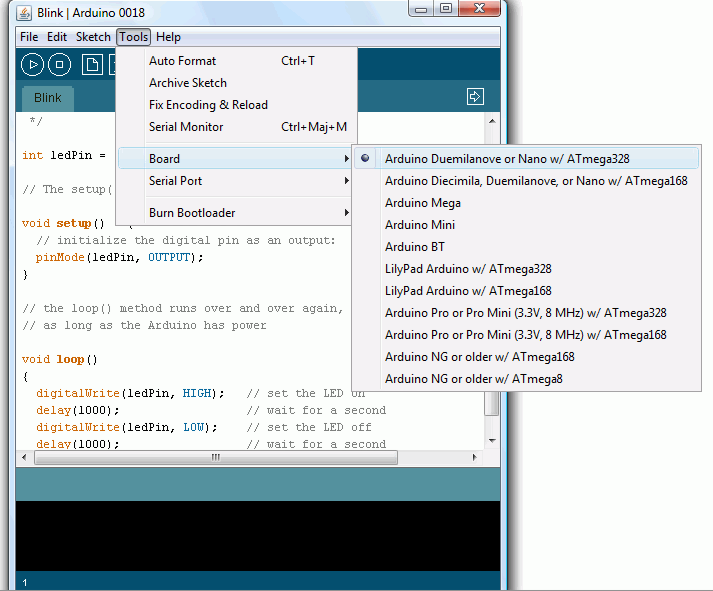
\includegraphics[scale=0.3]{../images/Arduino/logiciel.png}
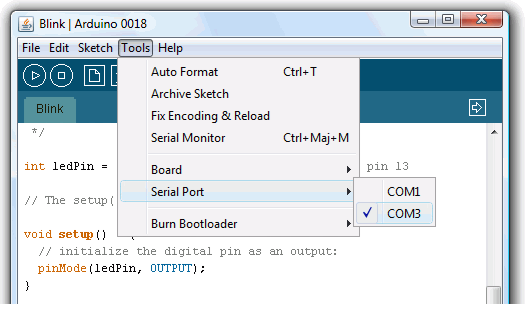
\includegraphics[scale=0.5]{../images/Arduino/logiciel1.png}
\caption{Environnement de travail: choix de la carte et du port}
\end{center}
\end{figure}

